\documentclass{article}
\usepackage{setspace}
\usepackage[utf8]{inputenc}
%\usepackage{subfigure}

\pagestyle{plain}

\usepackage{amssymb, bm, blkarray, multicol}
\usepackage{listings,xcolor,lmodern}
\usepackage{graphicx}
\usepackage{enumitem}
\usepackage{tikz}
\usepackage{booktabs}
\usepackage{amsmath}
\usepackage{algorithm}
\usepackage{algpseudocode}
\usepackage[nottoc]{tocbibind}
\usepackage{upgreek}

\usepackage{hyperref}
\usepackage{url}
\usepackage{nicefrac}
\usepackage{microtype}

\usepackage{latexsym}
% \usepackage{a4wide}

\newtheorem{theorem}{THEOREM}
\newtheorem{lemma}[theorem]{LEMMA}
\newtheorem{corollary}[theorem]{COROLLARY}
\newtheorem{proposition}[theorem]{PROPOSITION}
\newtheorem{remark}[theorem]{REMARK}
\newtheorem{definition}[theorem]{DEFINITION}
\newtheorem{fact}[theorem]{FACT}

\newtheorem{problem}[theorem]{PROBLEM}
\newtheorem{exercise}[theorem]{EXERCISE}
\def \set#1{\{#1\} }

\lstset{
  basicstyle=\ttfamily,
  columns=fullflexible,
  frame=single,
  breaklines=true,
  postbreak=\mbox{\textcolor{red}{$\hookrightarrow$}\space},
}

\newcommand{\E}{\mathbb{E}}
\newcommand{\var}{\mathrm{Var}}
\newcommand{\cov}{\mathrm{Cov}}
\newcommand{\KL}{\mathrm{KL}}
\newcommand{\neighb}{\text{ne}}
\DeclareMathOperator*{\argmax}{arg\,max}
\DeclareMathOperator*{\argmin}{arg\,min}
\newcommand{\Perp}{\mathrel{\text{\scalebox{1.07}{$\perp\mkern-10mu\perp$}}}}

\usetikzlibrary{shapes.geometric}

\title{  	{ 
\includegraphics[scale=.5]{figures/ucl_logo.png}}\\
{{\Huge Project Title}}\\
{\large Optional Subtitle}\\
		}
\date{Submission date: 11 September 2020}
\author{Andrew Wei Jiang \thanks{
{\bf Disclaimer:}
This report is submitted as part requirement for the MSc in Computational Statistics and Machine Learning at UCL. It is
substantially the result of my own work except where explicitly indicated in the text. The report may be freely copied and distributed provided the source is explicitly acknowledged.
\newline}
\\ \\
\\ \\
Supervisor's name}

\begin{document}
\maketitle
\thispagestyle{empty}
\onehalfspacing

\newpage
\begin{abstract}
    In Bayesian statistics, Markov chain Monte Carlo (MCMC) algorithms provide flexible ways to sample from analytically intractable posterior distributions. They are applied in a diverse collection fields ranging from statistical physics to evolutionary biology. However, inferences based on MCMC methods suffer from two sources of error: lack of convergence and mistakes in implementation. While there are a variety of methods to detect the former, less attention has been devoted to the latter. We propose two new tests for diagnosing MCMC implementation errors based on Maximum Mean Discrepancy (MMD). They  exhibit lower Type I/II error rates than the commonly used Geweke test \cite{geweke_getting_2004} and perform competitively with recently proposed alternatives in several experiments. However, the computational costs of both MMD tests are quadratic in the number of observations rather than linear. Finally, we provide some evidence that, unlike existing alternatives, the MMD tests can be generalized to domains other than $\mathbb{R}^{d}$.
\end{abstract}
\setcounter{page}{1}
\newpage

\tableofcontents
\newpage

\section{Introduction}
Convergence diagnostics \cite{gelman_inference_1992}, \cite{geweke_evaluating_1991}

Mistakes in MCMC \cite{del_negro_time_2015}

\section{Background}
TODO:
\begin{itemize}
    \item MCMC CLT and testing
    \item Reversible jump MCMC
    \item Two sample problem
    \item Alternative tests
    \item U / V statistics? asymptotics
    \item Kernel examples - Gaussian and linear
    \item $\tau$ dependence
    \item Wild bootstrap assumption
\end{itemize}

\subsection{Markov Chain Monte Carlo (MCMC)}
In Bayesian inference, given the prior distribution of the parameters $P(\mathbf{\Theta})$ and the likelihood of the observed data $P(\mathbf{Y} | \mathbf{\Theta})$, we are specifically interested in sampling from the posterior distribution 
\begin{equation}
    P(\mathbf{\Theta} | \mathbf{Y}) = \frac{P(\mathbf{Y} | \mathbf{\Theta})P(\mathbf{\Theta})}{P(\mathbf{Y})} \propto P(\mathbf{Y} | \mathbf{\Theta})P(\mathbf{\Theta})
    \label{eq:posterior}
\end{equation}
When the normalizer $P(\mathbf{Y})$ is analytically intractable, directly sampling from $P(\mathbf{\Theta} | \mathbf{Y})$ is impossible. Rather than drawing independent samples directly from a target distribution $P$, however, Markov chain Monte Carlo (MCMC) algorithms draw dependent samples from a Markov chain with stationary distribution $P$. The advantage of this approach is that it requires the density of $P$ to be known only up to a constant of proportionality. On the other hand, due to serial dependence and convergence time, a greater number of samples are required relative to independent sampling schemes in order to achieve the same performance, e.g., as measured by standard error if the objective is to calculate the expectation.

Other than in their target distributions, MCMC algorithms differ primarily in how they construct their Markov chains. Several methods are detailed below.

\subsubsection{The Metropolis-Hastings Algorithm}
Most MCMC algorithms use the Metropolis-Hastings algorithm can be used to construct a Markov chain with the desired stationary distribution (\cite{metropolis_equation_1953}, \cite{hastings_monte_1970}). Let $T(\mathbf{X} \rightarrow \mathbf{X}')$ denote the transition probability from state $\mathbf{X}$ to $\mathbf{X'}$ for an ergodic Markov chain $\{\mathbf{X}_{1}, \mathbf{X}_{2}, \ldots\}$. If $P$ satisfies the detailed balance condition
\begin{equation}
   T(\mathbf{X} \rightarrow \mathbf{X}') P(\mathbf{X}) = T(\mathbf{X}' \rightarrow \mathbf{X}) P(\mathbf{X}')
   \label{eq:dbc}
\end{equation}
then $\{\mathbf{X}_{1}, \mathbf{X}_{2}, \ldots\}$ is reversible and has unique stationary distribution $P$. 

At every iteration, the algorithm draws a proposal $\mathbf{X}'$ from a proposal distribution $q$, which is required to have non-zero measure on the support of $P$. $\mathbf{X}'$ is accepted with probability $A(\mathbf{X}'|\mathbf{X})$. Let $q(\mathbf{X}'|\mathbf{X})$ denote the proposal probability. Each transition probability can be decomposed into the product of the probability of proposing the next state and the probability of accepting the proposal.
\begin{align*}
    T(\mathbf{X} \rightarrow \mathbf{X}') &= q(\mathbf{X}'|\mathbf{X}) A(\mathbf{X}'|\mathbf{X})
\end{align*}
Rearranging (\ref{eq:dbc}) and setting  $A(\mathbf{X}|\mathbf{X}')=1$, the acceptance probability is
\begin{equation}
    A(\mathbf{X}'|\mathbf{X}) = \min{\left(\frac{q(\mathbf{X}|\mathbf{X}')  P(\mathbf{X}') }{q(\mathbf{X}'|\mathbf{X})  P(\mathbf{X})}, 1\right)}
\end{equation}

\subsubsection{The Gibbs Sampling Algorithm}
In the Bayesian setting characterized by (\ref{eq:bayesian}), the Gibbs sampling algorithm, a common Metropolis-Hastings variant, updates one parameter (or a block of parameters) $\Theta_{i}$ at a time using the proposal distribution
\begin{equation}
    q(\mathbf{\Theta}'|\mathbf{\Theta}, \mathbf{Y}) = P(\Theta_{i}' | \mathbf{\Theta}_{\neg i}, \mathbf{Y})
\end{equation}
Each proposal $\mathbf{\Theta}' = (\Theta_{i}', \mathbf{\Theta}_{\neg i}) $ is always accepted, since
\begin{equation}
    \begin{aligned}
    A(\mathbf{\Theta}'|\mathbf{\Theta}) &= \min{\left(\frac{q(\mathbf{\Theta}|\mathbf{\Theta}', \mathbf{Y})  P(\mathbf{\Theta}'|\mathbf{Y}) }{q(\mathbf{\Theta}'|\mathbf{\Theta}, \mathbf{Y})  P(\mathbf{\Theta}| \mathbf{Y})}, 1\right)} \\
    &= \min{\left(\frac{P(\Theta_{i} | \mathbf{\Theta}_{\neg i}, \mathbf{Y})  P(\mathbf{\Theta}'|\mathbf{Y}) }{P(\Theta_{i}' | \mathbf{\Theta}_{\neg i}, \mathbf{Y})  P(\mathbf{\Theta}| \mathbf{Y})}, 1\right)} \\
    &= \min{\left(\frac{P(\mathbf{\Theta}, \mathbf{Y})  P(\mathbf{\Theta}', \mathbf{Y}) }{P(\mathbf{\Theta}', \mathbf{Y})  P(\mathbf{\Theta}, \mathbf{Y})}, 1\right)} = 1 \\
    \end{aligned}
\end{equation}
A single iteration of the Gibbs sampler sweeps through all of the parameters. Note that while each individual update satisfies detailed balance, the entire sweep generally does not, unless the updates are conducted in palindromic or random order \cite{geyer_practical_1992}.

\subsubsection{The Reversible-jump Algorithm}
The reversible jump algorithm \cite{green_reversible_1995} generalizes the Metropolis-Hastings algorithm to allow `jumps' between spaces with different dimensions. This is particularly useful in a Bayesian model averaging context.



\subsection{Statistical Hypothesis Testing}
This section follows \cite{casella_statistical_1990} Chapter 8 and \cite{lehmann_testing_2005} Chapter 9. 
\begin{definition}[Two-sample Test]
    Given metric space $(M, d)$, let P and Q be two Borel probability measures defined on $M$, and let random variables $X$ and $Y$ be distributed as $X \sim P$ and $Y \sim Q$. Given samples $\{X_{i}\}_{i=1}^{N_{x}}$, $\{Y_{i}\}_{i=1}^{N_{y}}$, a statistical test $\mathcal{T}(\{X_{i}\}_{i=1}^{N_{x}}, \{Y_{i}\}_{i=1}^{N_{y}}): M^{N_{X}} \times M^{N_{Y}} \rightarrow \{0, 1\}$ distinguishes between the null hypothesis $H_{0}: P=Q$ and the alternative hypothesis $H_{1}: P \neq Q$.
\end{definition}
$\mathcal{T}$ compares a test statistic $s$ of the samples to a threshold $c_{\alpha}$, which is determined by design parameter (significance level) $\alpha$. If the statistic exceeds the threshold, then $\mathcal{T}$ rejects the null hypothesis; otherwise, it fails to reject $H_{0}$. Thus, the rejection region is $S_{\alpha} = \{s | s > c_{\alpha}\}$. Put another way, the test rejects $H_{0}$ when its p-value $p(s)=\inf \{\alpha | s \in S_{\alpha}\}$ is less than $\alpha$. To compare different tests, we consider their error rates.
\begin{definition}[Type I and Type II Errors]
    A Type I error is made when $H_{0}$ is true, but rejected by test $\mathcal{T}$. A Type II error is made when $H_{1}$ is true, but $\mathcal{T}$ fails to reject $H_{0}$.
\end{definition}
If $\mathcal{T}$ is consistent, in the large-sample limit, its Type I error rate is upper bounded by $\alpha$ and its Type II error rate is zero. An alternative metric to Type II error is test power, defined as $1-\beta$, where $\beta$ is the Type II error rate. In general, we want to minimize both error rates (minimizing the Type II error rate is equivalent to maximizing test power).

\subsubsection{Multiple Testing Corrections}
\begin{definition}[Family-wise Error Rate]
    Given a family of $N$ tests $\{\mathcal{T}_{i}\}_{i=1}^{N}$, the Family-wise Error Rate (FWER) is the probability that at least one test commits a Type I error.
\end{definition}
When testing multiple hypotheses, the FWER is analogous to the Type I error rate of a single test. When comparing families of tests to single tests later on, we will refer to both as Type I error rates. 

For a fixed significance level $\alpha$, it is well known that the FWER grows with the size of the associated family of tests --- however, this behavior can result in the inconsistency of the family. There are numerous procedures to address this. The simplest, known as the Bonferroni procedure \cite{bonferroni_il_nodate}, divides the significance level used for each individual test by the number of tests in the family. 

However, direct control of the FWER tends to reduce test power. Alternative procedures sacrifice some control of the FWER to combat this; these methods instead target the False Discovery Rate (FDR), defined as the proportion of rejected null hypotheses that are incorrectly rejected. When all null hypotheses are true, FDR is equivalent to FWER. One such approach is the Benjamini-Hochberg procedure \cite{benjamini_controlling_1995}

\begin{enumerate}
    \item Calculate p-values $\{p_{i}\}_{i=1}^{N}$, sorted in ascending order, for family $\{\mathcal{T}_{i}\}_{i=1}^{N}$
    \item Calculate $k = \sup \{i | \frac{i}{N} p_{k} \leq \alpha \} $
    \item Reject $\mathcal{H}_{0}^{i}$ for $i \leq k$
\end{enumerate}
which we will use for all multiple testing corrections in this study.

\subsection{Integration Tests for MCMC}
\subsubsection{Geweke Test for MCMC}
A commonly used diagnostic for MCMC samplers is the Geweke test \cite{geweke_getting_2004}. Given the model
\begin{align}
    P(\mathbf{Y}, \mathbf{\Theta}) = P(\mathbf{Y} | \mathbf{\Theta}) P(\mathbf{\Theta})
    \label{eq:bayesian}
\end{align}

The main idea is that there are multiple ways to generate samples from the joint distribution $P(\mathbf{\Theta}, \mathbf{Y})$. We can draw from the prior $P(\mathbf{\Theta})$ and then the likelihood $P(\mathbf{Y}| \mathbf{\Theta})$. Alternatively, we can alternate between drawing from the likelihood $P(\mathbf{Y}| \mathbf{\Theta})$ and the posterior $P(\mathbf{\Theta}|\mathbf{Y})$. If the sampling algorithms are correct, the resulting empirical distributions should be indistinguishable. To (indirectly) test this null hypothesis, we define some test functions of the samples and make use of the MCMC central limit theorem.

\begin{definition}[Test Function]
    Let $\mathbf{\Uptheta}$ denote the space of parameters and $\mathcal{Y}$ the space of the data in (\ref{eq:bayesian}). A test function satisfies $g:\mathrm{\Theta} \times \mathcal{Y} \rightarrow \mathbb{R}$ such that $\var(g(\mathbf{\Theta}, \mathbf{Y})) < \infty$. 
\end{definition}

Let $\mathbf{g}$ denote a vector of test functions. For each element of $\mathbf{g}$, the Geweke test compares two estimates of $\bar{g} = \E[g(\mathbf{\Theta}, \mathbf{Y})]$ using samples from Algorithms \ref{alg:mc-sampler} and \ref{alg:sc-sampler}.

\begin{algorithm}[H]
    \centering
    \caption{Marginal-conditional (MC) joint simulator}\label{alg:mc-sampler}
    \begin{algorithmic}[1]
        \State \text{Initialize} $\mathbf{g}_{MC} \in \mathbb{R}_{N\times |\mathbf{g}|}$
        \For{$n = 1, \ldots, N$}
            \State $\mathbf{\Theta}_{n} \sim P(\mathbf{\Theta})$ 
            \State $\mathbf{Y}_{n} \sim P(\mathbf{Y}|\mathbf{\Theta}_{n})$ 
            \State $\mathbf{g}_{MC}[n, :] = g(\mathbf{\Theta}_{n}, \mathbf{Y}_{n})$ 
        \EndFor        
        \State \textbf{return} $\mathbf{g}_{MC}$
    \end{algorithmic}
\end{algorithm}

\begin{algorithm}[H]
    \centering
    \caption{Successive-conditional (SC) joint simulator}\label{alg:sc-sampler}
    \begin{algorithmic}[1]
        \State \text{Initialize} $\mathbf{g}_{SC} \in \mathbb{R}_{N\times |\mathbf{g}|}$
        \State $\mathbf{\Theta}_{0} \sim P(\mathbf{\Theta})$ 
        \For{$n = 1, \ldots, N$}
            \State $\mathbf{Y}_{n} \sim P(\mathbf{Y}|\mathbf{\Theta}_{n-1})$ 
            \State $\mathbf{\Theta}_{n} \sim \text{PosteriorSampler}(\mathbf{\Theta}_{n-1}, \mathbf{Y}_{n})$ 
            \State $\mathbf{g}_{SC}[n, :] = \mathbf{g}(\mathbf{\Theta}_{n}, \mathbf{Y}_{n})$ 
        \EndFor        
        \State \textbf{return} $\mathbf{g}_{SC}$
    \end{algorithmic}
\end{algorithm}

In particular, 
\begin{equation}
    \frac{\hat{\bar{g}}_{MC} - \hat{\bar{g}}_{SC}}{\sqrt{ \frac{\hat{\sigma}^{2}_{MC}}{N_{MC}} + \frac{\hat{\sigma}^{2}_{SC}}{N_{SC}}}} \xrightarrow[]{d} \mathcal{N}(0, 1)
    \label{eq:geweke}
\end{equation}
with the mean estimates
\begin{align*}
    \hat{\bar{g}}_{MC} = \frac{1}{N_{MC}}\sum_{n=1}^{N_{MC}}g_{MC}^{(n)}, \qquad \hat{\bar{g}}_{SC} = \frac{1}{N_{SC}}\sum_{n=1}^{N_{SC}}g_{SC}^{(n)}
\end{align*}
The variance estimate for the marginal-conditional samples is straightforward
\begin{align*}
    \hat{\sigma}_{MC}^{2} = \frac{1}{N_{MC}}\sum_{n=1}^{N_{MC}}(g_{MC}^{(n)} - \hat{\bar{g}}_{MC})^{2}
\end{align*}
However, the successive-conditional variance estimate is not so simple, since the samples are dependent. Following \cite{geweke_using_1999}, we use the triangular window estimator
\begin{align*}
    \hat{\sigma}_{SC}^{2} &= \frac{1}{N_{SC}}\sum_{t=-\infty}^{\infty} w(t) \hat{\gamma}(t) \\
    \hat{\gamma}(t) &= \hat{\gamma}(-t) = \frac{1}{N_{SC}}\sum_{i=1}^{N_{SC}-t}(g_{SC}^{i} - \hat{\bar{g}}_{SC})(g_{SC}^{i+t} - \hat{\bar{g}}_{SC}) \\
    w(t) &= \max{\left(\frac{L-|t|}{L}, 0\right)}, \quad L \in \{0.04, 0.08, 0.15\} \times N
\end{align*}
See \cite{priestley_spectral_1981} for more on window functions.

For a given significance level $\alpha$, the testing procedure is
\begin{enumerate}
    \item Define test functions $\mathbf{g}$
    \item Draw $\mathbf{g}_{MC}, \mathbf{g}_{SC}$
    \item Calculate the left side of (\ref{eq:geweke}) for each test function element of $\mathbf{g}_{MC}, \mathbf{g}_{SC}$
    \item If any $|z| \geq \Phi^{-1}(1-\frac{\alpha}{2})$, reject the null hypothesis that the distributions are the same
\end{enumerate}

A reasonable selection of test functions is the set of all first and second empirical moments of the samples \cite{geweke_getting_2004}. In order to control the test's Type I error, it is important to correct for multiple testing, e.g., via Bonferroni.

A related, less principled approach is to examine the PP plot of the empirical MC and SC samples \cite{grosse_testing_2014}. If the points are far from the unit line, then we reject the null hypothesis.

\subsubsection{Alternative Tests for MCMC}
\cite{gandy_unit_2020}

\subsection{Reproducing Kernel Hilbert Space (RKHS)}
This section follows \cite{steinwart_support_2008}.

\begin{definition}[Hilbert Space]
    A vector space $\mathcal{H}$ over $\mathbb{R}$ is called a Hilbert Space if there exists a function $\langle \cdot, \cdot \rangle: \mathcal{H} \times \mathcal{H} \rightarrow \mathbb{R} $ satisfying
    \begin{enumerate}
        \item $\langle\alpha_{1} f_{1}+\alpha_{2} f_{2}, g\rangle_{\mathcal{H}}=\alpha_{1}\langle f_{1}, g\rangle_{\mathcal{H}}+\alpha_{2}\langle f_{2}, g\rangle_{\mathcal{H}}$ 
        \item $\langle f, g\rangle_{\mathcal{H}}=\langle g, f\rangle_{\mathcal{H}}$
        \item $\langle f, f\rangle_{\mathcal{H}} \geq 0$ and $\langle f, f\rangle_{\mathcal{H}}=0$ iff $f=0$
    \end{enumerate}
    $\forall f, f_{1}, f_{2},  g \in \mathcal{H}$. $\langle \cdot, \cdot \rangle$ is called an inner product.
    \label{def:hilbert_space}
\end{definition}

\begin{definition}[Kernel]
    Let $\mathcal{X}$ be a non-empty set. A function $k: \mathcal{X} \times \mathcal{X} \rightarrow \mathbb{R}$ is a kernel if there exists a Hilbert space $\mathcal{H}$ of real-valued functions on $\mathcal{X}$ and a feature map $\phi: \mathcal{X} \rightarrow \mathcal{H}$ such that $$ k(x, x') = \langle \phi(x), \phi(x') \rangle_{\mathcal{H}} \quad \forall x, x' \in \mathcal{X} $$
    Since $\phi(x) \in \mathcal{H}$ is a function, we may write $\phi(x)=k(\cdot, x)$. $k(\cdot, x)$ is called the canonical feature map.
\end{definition}

% Examples of kernels 

\begin{definition}[Reproducing Kernel Hilbert Space]
    A Hilbert space $\mathcal{H}$ is a Reproducing Kernel Hilbert Space (RKHS) if, for an associated kernel $k$
    \begin{enumerate}
        \item $k(\cdot, x) \in \mathcal{H} \quad \forall x \in \mathcal{X}$
        \item $\langle f, k(\cdot, x) \rangle_{\mathcal{H}} = f(x) \quad \forall f \in \mathcal{H}, x \in \mathcal{X} $ (reproducing property)
    \end{enumerate}
    $k(\cdot, \cdot)$ is called a reproducing kernel.
\end{definition}

\begin{definition}[Universal Kernel]
Let $\mathcal{Z}$ be a compact subset of $\mathcal{X}$, and let $C(\mathcal{Z})$ denote the space of all continuous functions from $\mathcal{Z}$ to $\mathbb{R}$. A continuous\footnote{By \cite{steinwart_uence_nodate} Lemma 3, a kernel is continuous iff its feature map is continuous} reproducing kernel $k$ on $\mathcal{Z}$ is universal if $\forall f \in C(\mathcal{Z}), \epsilon>0$, there exists a function in the associated RKHS $g \in \mathcal{H}$ such that 
$$ \Vert f-g \Vert_{\infty} \leq \epsilon $$
The associated RKHS of a universal kernel is called a universal RKHS \cite{steinwart_uence_nodate}.
\end{definition}

\begin{definition}[Mean embedding]
The mean embedding $\mu_{P}$ in RKHS $\mathcal{H}$ of a distribution $P$ is defined as 
    \begin{equation}
        \mathbf{\mu}_{P}(t) = \E_{P}[k(X, t)]
    \end{equation}    
    In particular $\mu_{P} \in \mathcal{H}$ satisfies
    \begin{equation}
        \E_{P}[f(X)] = \langle \mathbf{\mu}_{P}, f \rangle_{\mathcal{H}}
    \end{equation}
\end{definition}
The empirical estimate of the mean embedding is 
\begin{equation}
    \hat{\mathbf{\mu}}_{P}(t) = \frac{1}{N}\sum_{i=1}^{N}\phi(x_{i})
\end{equation}

\subsection{Maximum Mean Discrepancy (MMD)}
This discussion follows \cite{gretton_kernel_2012}. The workhorse of the tests we will present later is 
\begin{definition}[Maximum Mean Discrepancy (MMD)]
Let $\mathcal{F}$ be a space of functions $f:\mathcal{X}\rightarrow \mathbb{R}$, where $\mathcal{X}$ is a non-empty set. Then the Maximum Mean Discrepancy (MMD) is defined as the integral probability metric
    \begin{equation}
        \mathrm{MMD}[\mathcal{F}, P, Q]=\sup _{f \in \mathcal{F}}\left(\mathbf{E}_{X}[f(X)]-\mathbf{E}_{Y}[f(Y)]\right)
    \label{eq:mmd}
    \end{equation}
\end{definition}
A biased estimate of the MMD using samples $\{X_{i}\}_{i=1}^{N_{x}}$, $\{Y_{i}\}_{i=1}^{N_{y}}$ is
\begin{equation}
    \widehat{\mathrm{MMD}}_{V}[\mathcal{F}, \{X_{i}\}_{i=1}^{N_{x}}, \{Y_{i}\}_{i=1}^{N_{y}}]:=\sup _{f \in \mathcal{F}}\left(\frac{1}{N_{x}}\sum_{i=1}^{N_{x}}f(X_{i})-\frac{1}{N_{y}}\sum_{i=1}^{N_{y}}f(Y_{i})\right)
\end{equation}

When $\mathcal{F}$ is a unit ball on an RKHS $\mathcal{H}$ with associated kernel $k(\cdot, \cdot)$, the MMD admits the closed form
\begin{equation}
        \mathrm{MMD}[\mathcal{F}, P, Q] = \Vert \mathbf{\mu}_{P}-\mathbf{\mu}_{Q} \Vert_{\mathcal{F}}
    \label{eq:mmd_closed}
\end{equation}
and the biased empirical MMD can be computed via
\begin{equation}
        \widehat{\mathrm{MMD}}_{V}^{2} = \Vert \hat{\mathbf{\mu}}_{X}-\hat{\mathbf{\mu}_{Y}} \Vert_{\mathcal{F}} = \frac{1}{N_{x}^{2}} \sum_{i=1}^{N_{x}} \sum_{j=1}^{N_{x}} k\left(X_{i}, X_{j}\right)+\frac{1}{N_{y}^{2}} \sum_{i=1}^{N_{y}} \sum_{j=1}^{N_{y}} k\left(Y_{i}, Y_{j}\right)
        -\frac{2}{N_{x} N_{y}} \sum_{i=1}^{N_{x}} \sum_{j=1}^{N_{y}} k\left(X_{i}, Y_{j}\right)
        \label{eq:mmd_biased}
\end{equation}
which is the sum of two V-statistics and a sample average. An unbiased estimate can be obtained by exchanging the V-statistics for U-statistics
\begin{equation}
    \widehat{\mathrm{MMD}}_{U}^{2} = \frac{1}{{N_{x}\choose 2}} \sum_{i = 1}^{N_{x}} \sum_{i \neq i'}^{N_{x}} k\left(X_{i}, X_{i'}\right)+\frac{1}{{N_{y}\choose 2}} \sum_{j = 1}^{N_{y}} \sum_{j \neq j'}^{N_{y}} k\left(Y_{j}, Y_{j'}\right)-\frac{2}{N_{x}N_{y}} \sum_{i = 1}^{N_{x}} \sum_{j = 1}^{N_{y}} k\left(X_{i}, Y_{j}\right)
    \label{eq:mmd_unbiased}
\end{equation}
When $N_{x}=N_{y}=N$, (\ref{eq:mmd_biased}) and (\ref{eq:mmd_unbiased}) can be written as a one-sample V- and U-statistics, respectively
\begin{equation}
    \widehat{\mathrm{MMD}}_{V}^{2} = \frac{1}{N^{2}} \sum_{i, j} h(Z_{i}, Z_{j}) \label{mmd_u}
\end{equation}
\begin{equation}
    \widehat{\mathrm{MMD}}_{U}^{2} = \frac{1}{N(N-1)} \sum_{i \neq j} h(Z_{i}, Z_{j})
    \label{mmd_v}
\end{equation}
with $Z = (X, Y) \sim P \times Q$ and $h(Z_{i}, Z_{j})=k(X_{i}, X_{j}) + k(Y_{i}, Y_{j}) - k(X_{i}, Y_{j}) - k(X_{j}, Y_{i})$.

For a certain set of reproducing kernels, (\ref{eq:mmd}) is a metric on the space of probability distributions $M$, i.e. $\mathrm{MMD}[\mathcal{H}, P, Q]$ iff $P=Q$. Kernels that satisfy this property are called characteristic, and all universal kernels are also characteristic \cite{sriperumbudur_hilbert_nodate}.

Both the unbiased and biased estimates can be computed in quadratic time, and we will make use of them here. It should be noted that linear time versions also exist; however, their speed comes at the cost of higher variance and reduced power of related tests \cite{gretton_kernel_2012}.

% For even $N$, the linear time unbiased estimate is
% \begin{equation}
%     \widehat{\mathrm{MMD}}_{U, \mathrm{l}}^{2}(X, Y) = \frac{2}{N} \sum_{i=1}^{N/2} k(X_{2i-1}, X_{2i}) + k(Y_{2i-1}, Y_{2i}) - k(X_{2i}, Y_{2i-1}) - k(X_{2i-1}, Y_{2i})
% \end{equation}

\subsection{Dependent Wild Bootstrap}

Define the wild bootstrap process $\{W_{t,N}\}_{1\leq t\leq N}$ as
\begin{equation}
    W_{t, n}=e^{-1 / t_{n}} W_{t-1, n}+\sqrt{1-e^{-2 / l_{n}}} \epsilon_{t}
    \label{eq:wb_process}
\end{equation}
with $W_{0,N}, \epsilon_{t} \sim \mathcal{N}(0,1)$, satisfying the bootstrap assumption.

The bootstrapped MMD is
\begin{equation}
\begin{array}{c}
\widehat{\mathrm{MMD}}^{2}_{V, b}=\frac{1}{N_{x}^{2}} \sum_{i=1}^{N_{x}} \sum_{j=1}^{N_{x}} W_{i}^{(x)} W_{j}^{(x)} k\left(x_{i}, x_{j}\right)+\frac{1}{N_{y}^{2}} \sum_{i=1}^{N_{y}} \sum_{j=1}^{N_{y}} W_{i}^{(y)} W_{j}^{(y)} k\left(y_{i}, y_{j}\right) \\
\quad-\frac{2}{N_{x} N_{y}} \sum_{i=1}^{n_{s}} \sum_{j=1}^{N_{y}} W_{i}^{(x)} W_{j}^{(y)} k\left(x_{i}, y_{j}\right)
\end{array}
\label{eq:wb_mmd}
\end{equation}
We could also replace $W_{t}^{(x)}, W_{t}^{(y)}$ with their centered versions $\tilde{W}_{t}^{(x)}=W_{t}^{(x)}-\frac{1}{N_{x}} \sum_{i=1}^{N_{x}} W_{i}^{(x)}, \tilde{W}_{t}^{(y)}=W_{t}^{(y)}-\frac{1}{N_{y}} \sum_{j=1}^{N_{y}} W_{j}^{(y)}$; however, this tends to result in weaker control of Type I errors \cite{chwialkowski_wild_2016}.

Under the null hypothesis $P(X) = P(Y)$
\begin{equation*}
    \varphi\left(\rho_{x} \rho_{y} n \widehat{MMD}_{V}^{2}, \rho_{x} \rho_{y} n \widehat{MMD}^{2}_{V, b}\right) \xrightarrow[]{p} 0, \quad n\rightarrow \infty
\end{equation*}
where $\rho_{x} = \frac{N_{x}}{N_{x} + N_{y}}$, $\rho_{y} = \frac{N_{y}}{N_{x} + N_{y}}$.

\section{MMD Tests}
Though the Geweke test has been tried and tested, it suffers from several major limitations. First, it is unable to directly test the null hypothesis of interest, i.e., the joint distributions $P(\mathbf{Y}, \mathbf{\Theta})$ and $Q(\mathbf{Y}, \mathbf{\Theta})$ are the same. Instead, it requires us to first anticipate dimensions in which the distributions may differ, and then test hypotheses concerning those dimensions only. If we select too few test functions, the number of errors we cannot detect will be too high. On the other hand, if we select too many test functions, correcting for multiple testing may hamstring test power. Second, the test is limited to joint probability distributions on $\mathbb{R}^{d}$. Posterior samplers of other distributions, e.g., of graphs, cannot be checked without significant feature engineering. Third, drawing enough samples from Algorithm \ref{alg:sc-sampler} to offset their serial dependence may require significant computation that is difficult to parallelize beyond low-level matrix operations, though this dependence may also benefit test power by magnifying subtle errors in the sampler \cite{grosse_testing_2014}. 

We propose two two-sample MMD-based tests that address the first two limitations. Instead of manually specifying many test functions, we specify a kernel, and test functions (features) are implicit. Rather than conducting many indirect tests to approximately determine if two joint distributions are equal, we can test the null hypothesis $P=Q$ directly. In addition, as long as we can define a valid kernel and run Algorithm \ref{alg:mc-sampler}, we can conveniently check any MCMC sampler, even on graphs, strings, trees, etc. The test based on Algorithm \ref{alg:bc-sampler} addresses the third limitation and can be parallelized.

\subsection{Successive-conditional MMD Test}
The successive-conditional MMD (MMD-SC) test is similar to the Geweke test in that it uses Algorithms \ref{alg:mc-sampler} and \ref{alg:sc-sampler} to generate samples. The idea behind the MMD-SC test was briefly mentioned in \cite{lloyd_statistical_nodate}, and a similar test was applied in \cite{liu_kernelized_nodate} as a benchmark for model goodness-of-fit tests. However, our MMD-SC test differs in several ways. Most importantly, the former incorrectly uses the unbiased MMD test statistic (\ref{eq:mmd_unbiased}) with permutation bootstrapped null distribution. Because the MCMC samples are dependent, the permutation bootstrap assumption that the samples are i.i.d. is violated; in practice, this can result in elevated Type I error rates \cite{chwialkowski_wild_2016}. Instead, we use the biased MMD test statistic (\ref{eq:mmd_biased}) with wild bootstrapped null distribution, which allows for dependent samples \cite{chwialkowski_wild_2016}. The second difference is that the other test's MCMC algorithm requires a burn-in period to reach the stationary distribution, while Algorithm \ref{alg:sc-sampler} is initialized in the stationary distribution and no burn-in is required.

For significance level $\alpha$ and $B$ bootstrap samples, the testing procedure is
\begin{enumerate}
    \item Define test functions $\mathbf{g}(\mathbf{\Theta}, \mathbf{Y})$
    \item Draw $\mathbf{g}_{MC}, \mathbf{g}_{SC}$ using Algorithms \ref{alg:mc-sampler} and \ref{alg:sc-sampler} and normalize scale
    \item Calculate $\widehat{\mathrm{MMD}}_{V}^{2}$ on $\mathbf{g}_{MC}, \mathbf{g}_{SC}$
    \item Simulate $\{\rho_{1} \rho_{2} n \widehat{\mathrm{MMD}}^{2}_{V, b}\}_{b=1}^{B}$ using (\ref{eq:wb_mmd}) and calculate $c_{\alpha}$, their $1-\alpha$ empirical quantile
    \item If $\rho_{1} \rho_{2} n \widehat{MMD}^{2}_{V} \geq c_{\alpha}$, reject the null hypothesis that the distributions are the same
\end{enumerate}

\subsection{Backward-conditional MMD Test}
A major disadvantage of the successive-conditional sampler is that it cannot be parallelized because of the autocorrelation in the samples. The backward-conditional MMD (MMD-BC) test sidesteps this by drawing independent samples from the joint distribution $P(\mathbf{\Theta}, \mathbf{Y})$. To draw a single sample, we first draw $\mathbf{Y}_{i}$ from its marginal distribution, then run the posterior simulator to get $\mathbf{\Theta}_{i}$ after some burn-in. The entire process is shown in Algorithm \ref{alg:bc-sampler}. 

\begin{algorithm}[H]
    \centering
    \caption{Backward-conditional (BC) joint simulator}\label{alg:bc-sampler}
    \begin{algorithmic}[1]
        \State \text{Initialize} $\mathbf{g}_{BC} \in \mathbb{R}_{N\times |\mathbf{g}|}$
        \For{$n = 1, \ldots, N_{BC}$}
            \State $\mathbf{\Theta}_{0} \sim P(\mathbf{\Theta})$ 
            \State $\mathbf{Y}_{n} \sim P(\mathbf{Y}|\mathbf{\Theta}_{0})$ 
            \For{$m = 1, \ldots, M$}    
                \State $\mathbf{\Theta}_{n} \sim \text{PosteriorSampler}(\mathbf{\Theta}_{n}, \mathbf{Y}_{n})$
            \EndFor
            \State $\mathbf{g}_{BC}[n, :] = \mathbf{g}(\mathbf{\Theta}_{n}, \mathbf{Y}_{n})$ 
        \EndFor        
        \State \textbf{return} $\mathbf{g}_{BC}$
    \end{algorithmic}
\end{algorithm}

Since the samples are independent, we can then apply a test based on the unbiased MMD, using permutation bootstrapping to generate the null distribution as described in \cite{gretton_kernel_2012}. For a significance level $\alpha$ and $B$ bootstrap samples, the testing procedure is
\begin{enumerate}
    \item Define test functions $\mathbf{g}(\mathbf{\Theta}, \mathbf{Y})$
    \item Draw $\mathbf{g}_{MC}, \mathbf{g}_{BC}$ via Algorithms \ref{alg:mc-sampler} and \ref{alg:bc-sampler} and normalize scale
    \item Calculate $\widehat{\mathrm{MMD}}_{U}^{2}$ on $\mathbf{g}_{MC}, \mathbf{g}_{BC}$
    \item Simulate the null distribution of $\widehat{\mathrm{MMD}}_{U}^{2}$ via permutation and calculate the $1-\alpha$ empirical quantile $c_{\alpha}$
    \item If $\widehat{\mathrm{MMD}}_{U}^{2} \geq c_{\alpha}$, reject the null hypothesis that the distributions are the same
\end{enumerate}

\subsection{Test Functions}
Although MMD tests can in theory detect any difference between distributions given a characteristic kernel  \cite{gretton_kernel_2012}, they can benefit from the inclusion of intelligent test functions. In our experiments, following \cite{gandy_unit_2020}, we augment the samples with two additional test functions --- the evaluations of the likelihood $P(\mathbf{Y}|\mathbf{\Theta})$ and the prior $P(\mathbf{\Theta})$ on the sample. These features make intuitive sense in the MCMC setting. Under an incorrect posterior distribution, certain parameter values will be more or less likely to be observed than they would be under the correct posterior; since $P(\mathbf{\Theta}|\mathbf{Y}) \propto P(\mathbf{Y}|\mathbf{\Theta}) P(\mathbf{\Theta})$, these discrepancies should manifest in the likelihood and prior. The test functions used by the MMD tests are thus
\begin{equation}
    \mathbf{g}(\mathbf{\Theta}, \mathbf{Y}) = \begin{bmatrix} \mathbf{\Theta} & P(\mathbf{Y}|\mathbf{\Theta}) & P(\mathbf{\Theta}) \end{bmatrix}^{\top}
\end{equation}
As we will see in experiment 1, the additional features can have a dramatic effect on error detection.

\subsection{Kernel Selection}
In this study, since all our experiments can be cast as tests in $\mathbb{R}^{d}$, we will use the (characteristic, \cite{fukumizu_kernel_2007}) Gaussian kernel. There are a variety of methods in the literature for selecting the Gaussian kernel bandwidth. Though optimizing the t-statistic in \cite{sutherland_generative_2019} generally outperforms other methods for kernel parameter selection in terms of test power, this approach is relatively data-intensive, requiring a training set on which the parameters are learned. Because we assume drawing samples is expensive, we use the median heuristic, choosing the median pairwise distance in the pooled samples as the bandwidth.
% Citation?

If the feature scales of the sample differ by too much, the median heuristic may be inappropriate. Thus, before applying the heuristic, we first normalize the feature scales by dividing each sample feature by the corresponding pooled standard deviation.

\section{Experiments}
We will conduct three experiments to compare the performance of the successive-conditional and backward-conditional MMD tests (MMD-SC test and MMD-BC test, respectively) to the Geweke test as well as other benchmark tests, e.g., from \cite{gandy_unit_2020}, where appropriate.

When comparing tests, it is important to consider their varying computational costs as well as their Type I/II error rates. These costs can be decomposed into two components: the cost of drawing samples and the cost of running the test. While we would ideally calculate the performance of each test keeping total computational cost fixed, this can be quite difficult. It is tedious to enumerate all elementary operations involved; if we try to sidestep this issue by using compute time as a proxy as in \cite{gandy_unit_2020}, artificial discrepancies may arise from, e.g., CPU throttling or using libraries written in C++ in Python. Instead, we focus on keeping sampling costs approximately fixed across tests by counting the total number of samples they require from Algorithms \ref{alg:mc-sampler}, \ref{alg:sc-sampler}, or \ref{alg:bc-sampler}.

\subsection{Gibbs Sampling}
We first evaluate test performance on the Gibbs sampler from \cite{gandy_unit_2020}. The data generating process is
\begin{align}
    \theta_i &\sim \mathcal{N}(0, \sigma^2), \quad i=1,2 \\
    y &= \theta_1 + \theta_2 + \epsilon, \quad \epsilon \sim \mathcal{N}(0, \sigma_\epsilon^2)
\end{align}
By conjugacy, the Gibbs updates for $\mathbf{\theta}$ are
\begin{align}
\theta_{i} \sim \mathcal{N}\left(
\frac{\sigma^{2}}{\sigma_{\epsilon}^{2}+\sigma^{2}}\left(y-\theta_{j}\right)
, \frac{1}{\frac{1}{\sigma_{\epsilon}^{2}}+\frac{1}{\sigma^{2}}}\right), \quad i=1,2
\end{align}
The hyperparameters are set to $\sigma^{2}=100, \sigma_{\epsilon}^{2}=0.1$. Each iteration of the Gibbs sampler updates $\theta_{1}$ and $\theta_{2}$ in random order to preserve reversibility, which is required for the rank test.

Since the three errors introduced in \cite{gandy_unit_2020} are all either too easy to detect or unclearly described, we introduce two errors into the posterior sampler illustrating the importance of the auxiliary features. In the first error, the posterior distribution means are swapped. This is a plausible but subtle error; because the parameters are symmetric, the marginal distribution of the parameters is unchanged, and two-sample tests based solely on this marginal will fail to detect any error. In the second error, we replace the normal distributions in the Gibbs steps with Laplace distributions preserving the correct means and variance. These errors are summarized in Table \ref{tab:ex1_errors}.

\begin{table}[H]
    \centering
    \begin{tabular}{l|c|c|c}
         Error  & Components & Incorrect & Correct \\
         \hline
         Mean Swap & Means &  $\frac{\sigma^{2}}{\sigma_{\epsilon}^{2}+\sigma^{2}}\left(y-\theta_{i}\right)$ & $\frac{\sigma^{2}}{\sigma_{\epsilon}^{2}+\sigma^{2}}\left(y-\theta_{j}\right)$\\
         Laplace & Distributions & Laplace & Gaussian \\
    \end{tabular}
    \caption{Experiment 1 intentional errors in posterior sampler}
    \label{tab:ex1_errors}
\end{table}

First, we compare the performance of the MMD-BC test with the median-heuristic Gaussian kernel against the KS and Rank tests from \cite{gandy_unit_2020}. Each Type I/II error rate is calculated over 100 trials with $\alpha=0.05$ and all tests use the same sets of independent samples from Algorithms \ref{alg:mc-sampler} and \ref{alg:bc-sampler}, with $M=5$ for the BC sampler. The test functions used in each test are shown in Table \ref{tab:ex1_testfn}, and the results are plotted in Figure \ref{fig:ex1_aux}.

\begin{table}[H]
    \centering
    \begin{tabular}{l|c|c|c|c|c|c}
         Test  & $\theta_{1}$ & $\theta_{2}$ & $\theta_{1}^{2}$ & $\theta_{1}\theta_{2}$ & $P(\mathbf{y}|\mathbf{\theta})$ & $P(\mathbf{\theta})$ \\
         \hline
         MMD-SC & Y & Y & & & Y & Y \\
         MMD-BC & Y & Y & & & Y & Y \\
         Geweke & Y & Y & Y & Y & Y & Y \\
         KS & Y & Y & Y & Y & Y & Y \\
         Rank & Y & Y & Y & Y & Y & Y \\
    \end{tabular}
    \caption{Experiment 1 test functions}
    \label{tab:ex1_testfn}
\end{table}

\begin{figure}
    \centering
    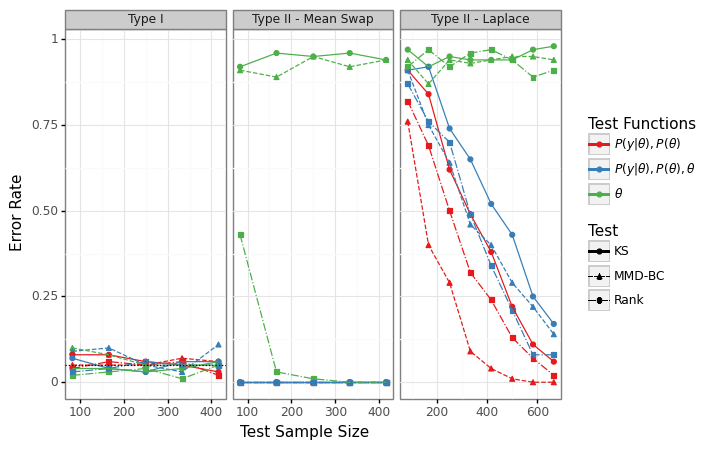
\includegraphics[width=\textwidth]{figures/gandy_scott_aux.png}
    \caption{Experiment 1 Type I/II error rates of BC tests with varying test functions, calculated over 100 trials with $\alpha=0.05$. The MMD-BC test used the Gaussian kernel with bandwidth set using the median heuristic, with scale-normalized data. The BC sampler set $M=5$. For the Rank test, we ordered test functions directly. For the MMD-BC and KS tests, `Test Sample Size' refers to the size of each sample seen by the tests. Though the Rank test is not a two-sample test, at a given `Test Sample Size', it runs roughly the same number of sampler iterations as the KS and MMD-BC tests.}
    \label{fig:ex1_aux}
\end{figure}

While the Type I error rates hover around the design parameter, without the auxiliary test functions, the Type II error rates for the KS and MMD-BC tests are stuck just below 1. This is a surprising result; the Gaussian kernel is characteristic on $\mathbb{R}^{d}$, but the test seems to require a very high number of samples to distinguish between the MC and BC distributions.

These errors were chosen to be difficult to detect in $\mathbf{\theta}$-space. Consequently, the auxiliary test functions appear to capture the greatest discrepancies between the MC and BC samples. In the Laplace Error, the inclusion of the $\mathbf{\theta}$ test functions visibly increases the Type II error across all tests, drastically in the MMD-BC test case. This illustrates the trade-off inherent in enumerating test functions. Loosely speaking, each additional test function drastically improves detection rates for errors along that dimension, but reduces detection rates for discrepancies along orthogonal or sufficiently "distant" dimensions. In the Geweke and KS tests, this reduction in detection rates is driven by the multiple testing correction applied. For the MMD tests, this reduction occurs because the similarity between observations increases when irrelevant features are added.

% Appendix?
To the extent that the benchmark tests rely on a finite set of test functions, they are only able to examine discrepancies in a limited number of nonlinear features. In contrast, MMD-based tests are able to account for an infinite number of nonlinear features when using particular nonlinear kernels. Figure \ref{fig:ex1_kernel} illustrates the resulting benefits to power for the MMD-BC test. 
\begin{figure}
    \centering
    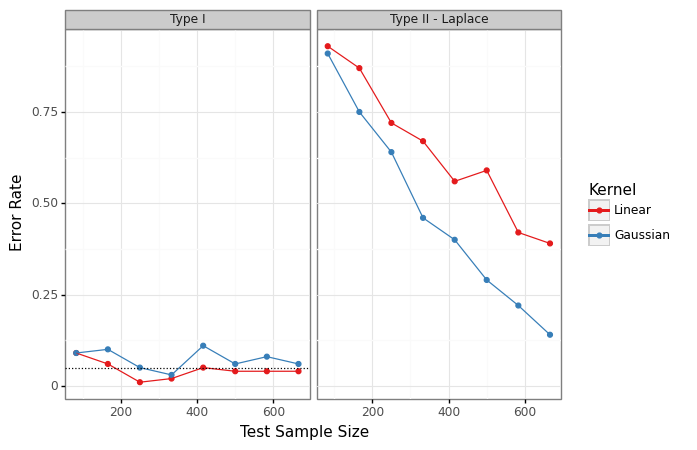
\includegraphics[width=\textwidth]{figures/gandy_scott_kernel.png}
    \caption{Experiment 1 MMD-BC Type I/II error rates using $\mathbf{\Theta}$ and the likelihood and prior auxiliary variables as test functions, calculated over 100 trials with $\alpha=0.05$. The BC sampler set $M=5$. We used Gaussian kernels with median heuristic bandwidths on scale-normalized data.}
    \label{fig:ex1_kernel}
\end{figure}

The autocorrelation in the SC samples is extreme; though the Type II error rates are close to zero for the given hyperparameters, the SC tests require far more samples than the BC tests to push the Type I error rate below $\alpha=0.05$. Comparing efficiency across test types is not meaningful for the default parameters. However, we can reduce the autocorrelation by increasing $\sigma_{\epsilon}$ to obtain a fairer comparison. Turning this knob will allow us to analyze how the tests behave given samplers with varying mixing speeds. 

In Figure \ref{fig:ex1_auto}, we plot the Type I/II error rates for the correct sampler and the Laplace error sampler, holding both the total sampler iterations used by each test and the test sample sizes fixed. As we might expect, when the sample autocorrelation is very high, the SC tests always reject the null hypothesis. As $\sigma_{\epsilon}$ increases and the autocorrelation falls, the SC Type I error rates fall. In this plot, the SC Type I error rates generally exceed the BC test Type I rates; this is caused by high autocorrelation in the successive-conditional chains. However, note that for a given $\sigma_{\epsilon}$, we can reduce the MMD-SC and Geweke Type I error rates by thinning the chains.

As the autocorrelation decreases and mixing improves, the Type II error rates tend to decrease across the board. The exception to this trend is the initial spike experienced by the SC tests. As we move right from the leftmost extreme ($\sigma_{\epsilon} = 0.1$), the autocorrelation weakens enough that the SC tests sometimes fail to reject the null. Notably, the MMD-SC test exhibits better control of Type I error rates than the Geweke test, despite the fact that both tests use the successive-conditional simulator (Algorithm \ref{alg:sc-sampler}). On the other hand, the MMD-SC test is also less likely to correctly reject the null hypothesis. For $\sigma_{\epsilon} \geq 2.5$, the MMD-SC test has similar Type II error rates to the MMD-BC test. The KS test's Type II error rates lag behind the other tests in this setting.

\begin{figure}[H]
    \centering
    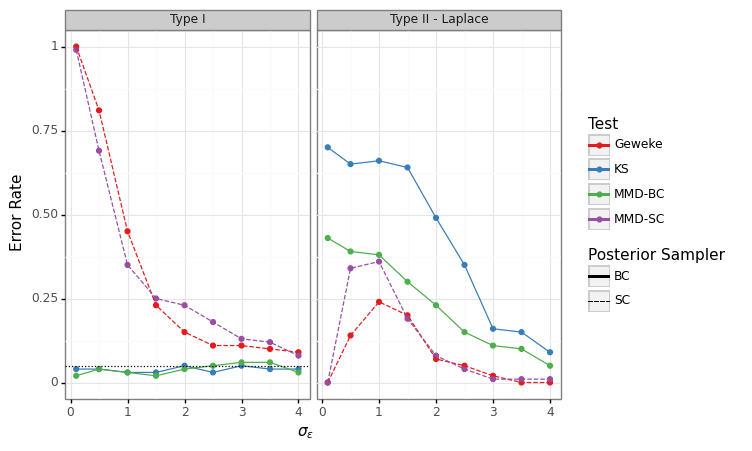
\includegraphics[width=\textwidth]{figures/gandy_scott_auto.png}
    \caption{Experiment 1 Type I/II error rates of BC and SC tests against $\sigma_{\epsilon}$, calculated over 100 trials with $\alpha=0.05$. As $\sigma_{\epsilon}$ increases, autocorrelation in the successive-conditional samples used in the Geweke and MMD-SC tests decreases. We allocated a budget of 1800 sampling iterations, keeping every 5th sample; each test received 300 samples from each sampler.}
    \label{fig:ex1_auto}
\end{figure}


\subsection{Reversible-jump Bayesian Lasso}
This example is based on \cite{chen_bayesian_2011}, but avoids using improper (hyper)priors in order to allow us to run Algorithm \ref{alg:mc-sampler}. We are interested in learning the parsimonious linear regression model
\begin{equation}
  \mathbf{y} = \mathbf{X}\mathbf{\beta} + \mathbf{\epsilon}, \quad \mathbf{\epsilon} \sim \mathcal{N}(\mathbf{0}, \sigma^{2} \mathbf{I})
\end{equation}
in a Bayesian setting. Rather than introducing an L1 penalty to the objective function with a corresponding regularization parameter as in frequentist Lasso, we instead promote sparsity by placing a truncated Poisson prior on the number $k$ of nonzero coefficients $\beta_{j}$, drawing $k$ coefficients from a Laplace distribution, and setting the remaining $p-k$ coefficients to zero. In addition, we place an inverse-gamma prior on $\sigma^{2}$. Let $\mathbf{\Theta} = \{\lambda, \sigma, k, \mathbf{\gamma}, \mathbf{\beta}\}$ denote the parameters, $\mathbf{X} \in \mathbb{R}^{n \times p}$ denote the (fixed) data, and $\mathbf{y} \in \mathbb{R}^{n \times 1}$ denote the data. The model is characterized by

\begin{equation}
  P(\mathbf{\Theta}|\tau, a, b ) = P(k|\lambda) P(\mathbf{\gamma}|k) P(\beta_{j} | \tau, \gamma) P(\sigma^{2} | a, b)
\end{equation}
\begin{equation}
  P(k|\lambda) = \frac{\exp{(-\lambda)} \lambda^{k}}{Ck!}, \quad k \in \{1,\ldots, p\}
\end{equation}
\begin{equation}
  P(\mathbf{\gamma}|k) = {p\choose k}^{-1}
\end{equation}
\begin{equation}
  P(\beta_{j} | \tau, \gamma ) = \begin{cases} (2\tau)^{-1}\exp(-\frac{|\beta_{j}|}{\tau}) & j \in \mathbf{\gamma} \\ \delta(\beta_{j}) & \text{otherwise} \end{cases}
\end{equation}
\begin{equation}
    P(\sigma^{2} | a, b) = \frac{b^{a}}{\Gamma(a)} (\sigma^{2})^{-a-1} \exp{\left(-\frac{b}{\sigma^{2}}\right)}
\end{equation}
where $C$ is a normalization constant, $\delta$ is the Dirac delta function, and $\mathbf{\gamma}$ is a vector of the nonzero indices of $\mathbf{\beta}$.

The likelihood is given by
\begin{equation}
  P(\mathbf{y} | \sigma, \mathbf{\beta}, \mathbf{X} ) = (2\pi)^{-\frac{n}{2}} \sigma^{-n} \exp{\left(-\frac{\Vert\mathbf{y}-\mathbf{X}\mathbf{\beta}\Vert^{2}_{2}}{2\sigma^{2}}\right)}
\end{equation}
The joint probability is then
\begin{equation}
    \begin{aligned}
         P(\mathbf{y}, \mathbf{\Theta} | \mathbf{X} ) \propto &\sigma^{-n} \exp{\left(-\frac{\Vert\mathbf{y}-\mathbf{X}\mathbf{\beta}\Vert^{2}_{2}}{2\sigma^{2}}\right)} \times \\ 
         & \frac{\exp{(-\lambda)} \lambda^{k}}{k!} {p\choose k}^{-1} \prod_{j\in \mathbf{\gamma}} (2\tau)^{-1}\exp(-\frac{|\beta_{j}|}{\tau}) \prod_{k \notin \mathbf{\gamma}} \delta(\beta_{k}) \frac{b^{a}}{\Gamma(a)} (\sigma^{2})^{-a-1} \exp{\left(-\frac{b}{\sigma^{2}}\right)}
    \end{aligned}
    \label{eq:ex2_joint}
\end{equation}

Each iteration of the reversible-jump MCMC posterior sampler takes two steps in random order. The first is a Gibbs step, which is straightforward due to the conjugacy of the Inverse Gamma prior on $\sigma^{2}$.
\begin{equation}
    \sigma^{2} | \mathbf{y}, \mathbf{X}, \mathbf{\beta} \sim \mathcal{IG}\left(a + \frac{n}{2}, b + \frac{\sum_{i=1}^{n}(y_{i}-\mathbf{x}_{i}\mathbf{\beta})^{2} }{2}\right)
\end{equation}
where $\mathbf{x}_{i}$ denotes row $i$ of $\mathbf{X}$.

The second is a more involved reversible jump step. We start by proposing $k' \in \{k-1, k, k+1\}$ uniformly at random, disallowing $k<1$ and $k>p$. Thus, when $k \in \{1,p\}$, there are only two valid proposals, not three. Then, depending on the $k'$ proposed, we complete the proposal $\mathbf{\Theta}'$ via one of the following
\begin{itemize}
    \item Update: $k' = k$
    \begin{enumerate}
        \item Choose $j \in \{1, \ldots, k\}$ uniformly at random
        \item Propose $\mathbf{\gamma}' = \mathbf{\gamma}, \beta'_{j} = \beta_{j} + \mathcal{N}(0, \epsilon_{\text{update}}), \beta'_{i \neq j} = \beta_{i}$
        \item $P(\mathbf{\Theta}' \rightarrow \mathbf{\Theta}) = P(\mathbf{\Theta} \rightarrow \mathbf{\Theta}')=\mathcal{N}(\beta_{j}'; \beta_{j},\epsilon_{\text{update}})=\mathcal{N}(\beta_{j}; \beta_{j}',\epsilon_{\text{update}})$
    \end{enumerate}
\end{itemize}

\begin{itemize}
    \item Birth: $k' = k+1$
    \begin{enumerate}
        \item Choose $j \in \{k+1, \ldots, p\}$ uniformly at random
        \item Propose $\mathbf{\gamma}' = \mathbf{\gamma} \cup j$
        \item Propose $\beta'_{j} = \mathcal{N}(0, \epsilon_{\text{birth}}), \beta'_{i \neq j} = \beta_{i}$
        \item $P(\mathbf{\Theta}' \rightarrow \mathbf{\Theta}) = \begin{cases}\frac{1}{2}\frac{1}{k'} & k'=p \\ \frac{1}{3} \frac{1}{k'} & 1<k<p \end{cases} $
        \item $P(\mathbf{\Theta} \rightarrow \mathbf{\Theta}') = \begin{cases}\frac{1}{2}\frac{1}{p-k} \mathcal{N}(\beta_{j}'; 0,\epsilon_{\text{birth}}) & k=1 \\ \frac{1}{3} \frac{1}{p-k} \mathcal{N}(\beta_{j}'; 0,\epsilon_{\text{birth}}) & 1<k<p \end{cases} $
    \end{enumerate}
\end{itemize}

\begin{itemize}
    \item Death: $k' = k-1$
    \begin{enumerate}
        \item Choose $j \in \{1, \ldots, k\}$ uniformly at random
        \item Propose $\mathbf{\gamma}' = \mathbf{\gamma} \setminus j$ 
        \item Propose $\beta'_{j} = 0, \beta'_{i \neq j} = \beta_{i}$
        \item $P(\mathbf{\Theta}' \rightarrow \mathbf{\Theta}) = \begin{cases}\frac{1}{2}\frac{1}{p-k'} \mathcal{N}(\beta_{j}; 0,\epsilon_{\text{birth}}) & k'=1 \\ \frac{1}{3} \frac{1}{p-k'} \mathcal{N}(\beta_{j}; 0,\epsilon_{\text{birth}}) & 1<k'<p \end{cases} $
        \item $P(\mathbf{\Theta} \rightarrow \mathbf{\Theta}') = \begin{cases}\frac{1}{2}\frac{1}{k} & k=p \\ \frac{1}{3} \frac{1}{k} & 1<k<p \end{cases} $
    \end{enumerate}
\end{itemize}
where $\epsilon_{\text{update}}, \epsilon_{\text{birth}}$ are random walk sizes. We accept proposal $\mathbf{\Theta}'$ with probability $$A(\mathbf{\Theta}'|\mathbf{\Theta}) = \min{\left(\frac{P(\mathbf{y}, \mathbf{\Theta'} | \mathbf{X} )}{P(\mathbf{y}, \mathbf{\Theta} | \mathbf{X} )} \frac{P(\mathbf{\Theta}' \rightarrow \mathbf{\Theta})}{P(\mathbf{\Theta} \rightarrow \mathbf{\Theta}')}, 1\right)}$$

For this experiment, we fix the data $\mathbf{X} \in \mathbb{R}^{1 \times 3}$, with $\lambda=1$ and hyperparameters $\tau=1, a=3, b=1$. The random walk sizes are set to $\epsilon_\text{update}= \epsilon_\text{birth}=1$.

We introduce several intentional errors into the the posterior sampler summarized in Table \ref{tab:ex2_errors}. The first error affects the Metropolis-Hastings acceptance probabilities used in the birth/death moves; it omits the jump probabilities $P(\mathbf{\Theta}' \rightarrow \mathbf{\Theta}), P(\mathbf{\Theta} \rightarrow \mathbf{\Theta}')$ from the calculation. The second error affects all of the Metropolis-Hastings acceptance probabilities. The $P(k|\lambda)$ factors of the joint probabilities have incorrect denominator $(k-1)!$ rather than $k!$.

\begin{table}[H]
    \centering
    \begin{tabular}{l|c|c|c}
          Error & Components & Incorrect & Correct \\
         \hline
         Transition & $A_{\text{birth}}(\mathbf{\Theta}'|\mathbf{\Theta})$, $A_{\text{death}}(\mathbf{\Theta}'|\mathbf{\Theta})$  &  $\min{\left(\frac{P(\mathbf{y}, \mathbf{\Theta'} | \mathbf{X} )}{P(\mathbf{y}, \mathbf{\Theta} | \mathbf{X} )}, 1\right)}$ & $\min{\left(\frac{P(\mathbf{y}, \mathbf{\Theta'} | \mathbf{X} )}{P(\mathbf{y}, \mathbf{\Theta} | \mathbf{X} )} \frac{P(\mathbf{\Theta}' \rightarrow \mathbf{\Theta})}{P(\mathbf{\Theta} \rightarrow \mathbf{\Theta}')}, 1\right)}$\\
         Poisson & $P(\mathbf{y}, \mathbf{\Theta'} | \mathbf{X} )$, $P(\mathbf{y}, \mathbf{\Theta} | \mathbf{X} )$ & $\ldots \frac{\exp{(-\lambda)} \lambda^{k}}{(k-1)!} \ldots$ & $\ldots \frac{\exp{(-\lambda)} \lambda^{k}}{k!} \ldots$ \\
    \end{tabular}
    \caption{Experiment 2 intentional errors in posterior sampler}
    \label{tab:ex2_errors}
\end{table}

The results are shown in Figure \ref{fig:ex2_comparison}, with test functions shown in Table \ref{tab:ex2_testfn}. The Type I error rates of the BC tests hover around the design parameter of $\alpha=0.05$, while the Geweke Type I error rates are elevated, at 19-25\%. The MMD-SC test has similar Type I error rates to the MMD-BC test. However, when centered wild bootstrap processes were used with the MMD-SC test (not shown), Type I error rates were elevated at around 9-13\%; this is consistent with observations in \cite{sutherland_generative_2019}. Note that these error rates, calculated using 100 trials, are relatively noisy.

\begin{table}[H]
    \centering
    \begin{tabular}{l|c|c|c|c}
         Test  & $\mathbf{\beta}, \sigma$ & $\{\mathbf{\beta}, \sigma\} \times \{\mathbf{\beta}, \sigma\}$ & $P(\mathbf{y}|\mathbf{\Theta}, \mathbf{X})$ & $P(\mathbf{\Theta})$ \\
         \hline
         MMD-SC & Y & & Y & Y \\
         MMD-BC & Y & & Y & Y \\
         Geweke & Y & Y & Y & Y \\
         KS & Y & Y & Y & Y \\
         Rank & Y & Y & Y & Y\\
    \end{tabular}
    \caption{Experiment 2 test functions}
    \label{tab:ex2_testfn}
\end{table}

For the two-sample tests, the Transition error is much easier to detect than the Poisson error, while the opposite is true for the Rank test.  Notably, while the Geweke test detects the Transition error quite easily, it essentially is unable to detect the Poisson error at the computation levels shown. In contrast, the other tests perform reasonably well, with Type II error rates that fall relatively quickly with sample size. 

Across both errors, we see that the MMD-SC test has lower Type II error rates than the MMD-BC test --- further evidence of the error magnification properties of Algorithm \ref{alg:sc-sampler}. The MMD-SC test most efficiently detects the Transition error, but lags behind the KS and Rank tests in detecting the Poisson error. The performance of the KS test is extremely efficient in both cases, which suggests that the errors may manifest themselves in the test functions not included in the MMD tests, i.e., the second moments of the parameters.

\begin{figure}[H]
    \centering
    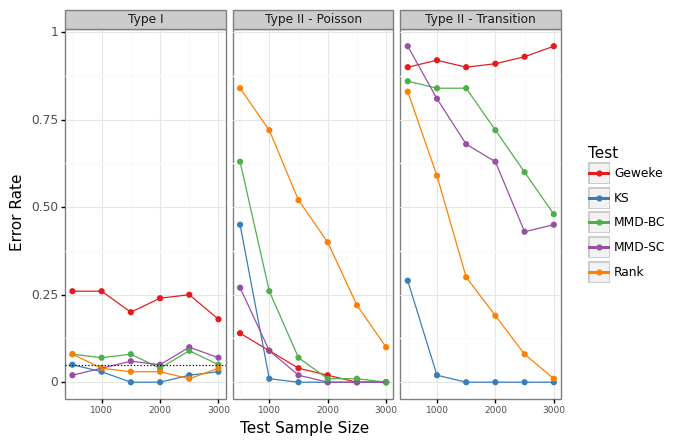
\includegraphics[width=\textwidth]{figures/bayes_lasso_comparison.png}
    \caption{Experiment 2 Type I/II error rates calculated over 100 trials with $\alpha=0.05$. Every 5 BC and SC samples were kept. The MMD tests used Gaussian kernels with median heuristic bandwidths on scale-normalized data.}
    \label{fig:ex2_comparison}
\end{figure}



\subsection{Metropolis-Hastings for Learning DAG Structure}
In this experiment, we are interested in learning the structure of a directed acyclic graph (DAG) given observed data. See Figure \ref{fig:ex3_dag} for an example of a DAG.

\begin{figure}[H]
    \centering
    \begin{minipage}[b]{0.25\textwidth}
        \centering
        \usetikzlibrary{shapes.geometric}
        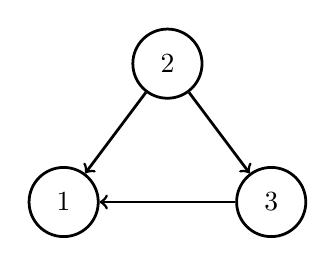
\begin{tikzpicture}
        [every node/.style={inner sep=0pt}]
        \node (1) [circle, minimum size=25.0pt, fill=white, line width=1pt, draw=black] at (112.5pt, -150.0pt) {\textcolor{black}{1}};
        \node (2) [circle, minimum size=25.0pt, fill=white, line width=1pt, draw=black] at (150.0pt, -100.0pt) {\textcolor{black}{2}};
        \node (3) [circle, minimum size=25.0pt, fill=white, line width=1pt, draw=black] at (187.5pt, -150.0pt) {\textcolor{black}{3}};
        \draw [line width=1, ->, color=black] (2) to  (1);
        \draw [line width=1, ->, color=black] (3) to  (1);
        \draw [line width=1, ->, color=black] (2) to  (3);
        \end{tikzpicture}
    \end{minipage}
     \begin{minipage}[b]{0.25\textwidth}
    \begin{align*}
        \begin{bmatrix}
            0 & 0 & 0 \\
            1 & 0 & 1 \\
            1 & 0 & 0 
        \end{bmatrix}
    \end{align*}
    \vspace{2ex}
    \end{minipage}
    \caption{Directed acyclic graph (DAG) with adjacency matrix representation. In the adjacency matrix, entry $(i,j)=1$ indicates the presence of a directed edge from node $i$ to node $j$; node $i$ is called a parent of $j$ and node node $j$ is called a child of node $i$. A node with no parents is called a root, and a node with no children is called a leaf.}
    \label{fig:ex3_dag}
\end{figure}

Let each observation on a root node $x_{r}$ be drawn from a normal distribution with standard deviation $\epsilon$, and let each child node be drawn from a normal distribution centered on the sum of its parents, also with standard deviation $\epsilon$. In other words, given graph structure $\mathcal{G}$ and data $\mathbf{X}$
\begin{equation}
    x_{r} \sim \mathcal{N}(0, \epsilon^2)
\end{equation}
\begin{equation}
    x_{j}|\mathbf{pa}(x_{j}) \sim \mathcal{N}(\sum_{z \in \mathbf{pa}(x_{j})} z, \epsilon^2)
\end{equation}
where $\mathbf{pa}(x)$ denotes the set of parent nodes of node $x$. Since the number of possible DAG structures is exponential in the number of nodes, for computational convenience, we consider all 3-node DAG structures.

Placing a uniform prior on $\mathcal{G}$, the posterior is proportional to the likelihood
\begin{equation}
    P(\mathcal{G}|\mathbf{X}) \propto P(\mathbf{X}|\mathcal{G}) = \prod_{i=1}^{n} \prod_{j=1}^{p} P(x_{ij}|\mathbf{pa}(x_{ij})) = \prod_{i=1}^{n} \prod_{j=1}^{p}
    \mathcal{N}(\sum_{z_{i} \in \mathbf{pa}(x_{ij})} z_{i}, \epsilon^2)
\end{equation}

The sampling algorithm we will consider is a modified version of the MCMC scheme from \cite{madigan_bayesian_1995} and is detailed in \cite{grzegorczyk_improving_2008}. Given a graph structure $\mathcal{G}_t$, the proposal structure is sampled uniformly from the neighborhood of $\mathcal{G}_t$
\begin{equation}
P(\mathcal{G}' | \mathcal{G}_t) = \frac{1}{|\mathbf{Ne}(\mathcal{G}_t)|}
\end{equation}
where the neighborhood $\mathbf{Ne}(\mathcal{G}_t)$ is defined as the union of $\mathcal{G}_t$ and the set of all DAGs that can be reached by adding, deleting, or reversing an edge.

The Metropolis-Hastings acceptance probability is thus
\begin{equation}
A(\mathcal{G}'|\mathcal{G}) = \min{\left(1,\frac{P(\mathbf{X}|\mathcal{G}')|\mathbf{Ne}(\mathcal{G}_t)|}{P(\mathbf{X}|\mathcal{G}_t)|\mathbf{Ne}(\mathcal{G}')|}\right)}
\end{equation}

The sampler errors considered all affect the Metropolis-Hastings acceptance probability; specifically, they alter the calculation of $|\mathbf{Ne}(\mathcal{G})|$. In the first error, we count all \textit{graphs} that can be reached by modifying a single edge, regardless of whether the modification induces a cycle. In the second error, we double-count the DAGs that can be reached by reversing an edge. These errors are summarized in Table \ref{tab:ex3_errors}.

\begin{table}
    \centering
    \begin{tabular}{l|c|c|c}
          Error & Components & Incorrect & Correct \\
         \hline
         Cyclic Check & $|\mathbf{Ne}(\mathcal{G}_t)|, |\mathbf{Ne}(\mathcal{G}_t)'|$ & Count all graphs & Count all DAGs \\
         Rev Count & $|\mathbf{Ne}(\mathcal{G}_t)|, |\mathbf{Ne}(\mathcal{G}_t)'|$ & Count edge reversals twice & Count reversals once \\
    \end{tabular}
    \caption{Experiment 3 intentional errors in posterior sampler}
    \label{tab:ex3_errors}
\end{table}

We compare the MMD tests against the benchmark Geweke and Rank tests, with each test using the same set of manually engineered test functions (features) in a subset of $\mathbb{R}^{d}$. The MMD tests again use the Gaussian kernel with median heuristic bandwidth calculated on scale-normalized inputs. As a final benchmark, we include a $\chi^{2}$ test of the sample DAG frequencies. 

Most of the features are derived from the adjacency matrix representation of the sampled graph structure $\mathcal{G}$, shown in Figure \ref{fig:ex3_dag}. As an initial set of features, we take
take each entry $(i,j)$, each $\mathrm{AND}((i,j),(i',j'))$, and each $\mathrm{XOR}((i,j),(i',j'))$ for all $i,j,i',j'$. We then prune features that are constant by construction or exactly equal to other features. First, we remove features derived from duplicate pairs, e.g., we keep only one of \{$\mathrm{AND}((i,j),(i',j'))=0$, $\mathrm{AND}((i',j'),(i,j))=0$\}. Next, diagonal entries $(i,i)=0$ are excluded (if they are nonzero, the graph is cyclic), along with all features derived from pairs with at least one diagonal entry. We also exclude $\mathrm{AND}((i,j),(j,i))=0$ and $\mathrm{XOR}((i,j),(i,j))=0$. Finally, we remove $\mathrm{AND}((i,j),(i,j)) = (i,j)$. As in the previous experiments, we also include the evaluation of the likelihood $P(\mathbf{Y}|\mathcal{G})$; the evaluation of the uniform prior $P(\mathcal{G})$ is omitted because it is constant.

The results are shown in Figure \ref{fig:ex3_comparison}. Type I error rates are approximately what we would expect from the design parameter.

It is clear that the Rank test is inappropriate for this setting; it is unable to detect either error. For the other tests, the Cyclic Check error is much easier to detect than the Rev Count error. 

The $\chi^{2}$ test generally has the best detection rates, likely due to the fact that it operates directly on the space of DAGs rather than an incomplete representation in $\mathbb{R}^{d}$. Surprisingly, however, the MMD-SC test comes quite close to matching its ability to detect the Cyclic Check error. In the Rev Count error, the SC tests slightly lead the MMD-BC test in performance and match the $\chi^{2}$ test. Finally, we see once more that the MMD-SC test has lower Type II error rates than the MMD-BC test.

\begin{figure}[H]
    \centering
    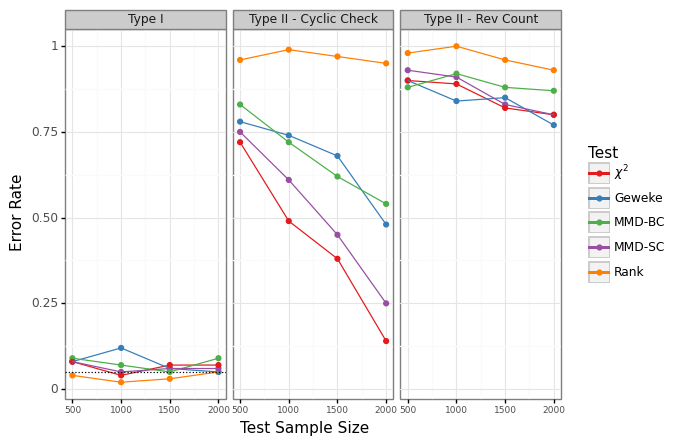
\includegraphics[width=\textwidth]{figures/graph_comparison.png}
    \caption{Experiment 3 Type I/II error rates calculated over 100 trials with $\alpha=0.05$. Every 5 BC and SC samples were kept. The MMD tests used Gaussian kernels with median heuristic bandwidths on scale-normalized data. For the Rank test, we ordered test functions directly using a random tiebreak.}
    \label{fig:ex3_comparison}
\end{figure}

Another question we may ask is how much the use of a nonlinear kernel in the MMD tests buys us here, given that all but one of the features used are binary. Figure \ref{fig:ex3_kernel} suggests that the gains can be substantial. In the case of the Cyclic Check error, using the Gaussian kernel improves Type II by around 8\% across both tests. The effect on the Rev Count Type II error is unclear.

\begin{figure}[H]
    \centering
    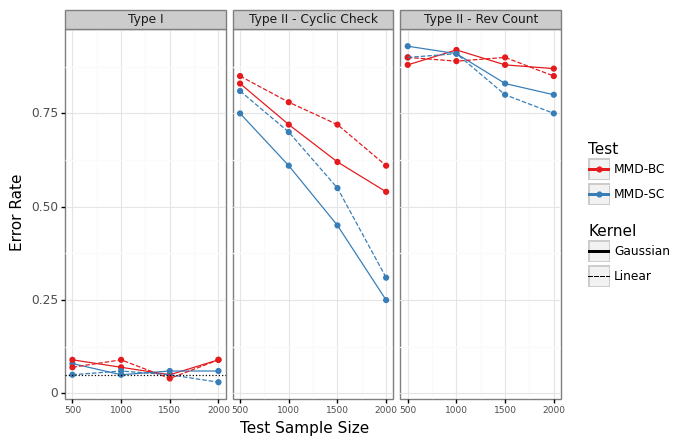
\includegraphics[width=\textwidth]{figures/graph_kernel.png}
    \caption{Experiment 3 Type I/II error rates for MMD tests using linear/nonlinear kernels. Calculated over 100 trials with $\alpha=0.05$. Every 5 BC and SC samples were kept.}
    \label{fig:ex3_kernel}
\end{figure}

It is important to emphasize that the tests as formulated are generally too expensive to conduct in richer DAG spaces; see the section \ref{section:discussion} for more details. It is possible, however, to adapt the MMD tests to these settings by using graph kernels; see \cite{kriege_survey_2020} for a survey. As a proof of concept we ran this experiment using random walk kernels \cite{gartner_graph_2003}, \cite{vishwanathan_fast_2006} in Figure \ref{fig:ex3_rw}. The kernels did not include any of our auxiliary test functions; combining data from different domains is another issue entirely. Using the random walk kernel, the MMD tests are able to detect the Cyclic Check error better than the $\chi^{2}$ test; however, the Rev Count Type II error degrades. In fact, random walk kernels cannot distinguish between isomorphic graphs. This illustrates a central issue with MMD; if a characteristic kernel is unavailable, MMD is not a metric on the space of probability distributions, and we will be unable to detect some differences between distributions.
\begin{figure}[H]
    \centering
    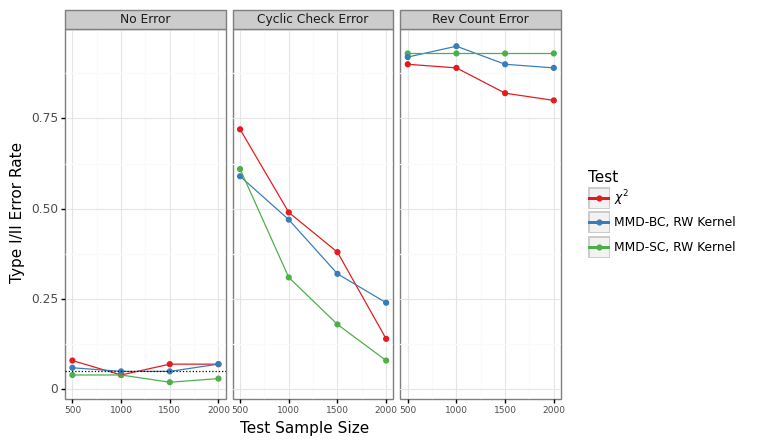
\includegraphics[width=\textwidth]{figures/graph_random_walk.png}
    \caption{Experiment 3 Type I/II error rates for MMD tests using the GraKeL \cite{siglidis_grakel_2020} random walk kernel implementation, with $\lambda=0.1$ and `geometric' summation. Calculated over 100 trials with $\alpha=0.05$. Every 5 BC and SC samples were kept.}
    \label{fig:ex3_rw}
\end{figure}

\section{Discussion}
\label{section:discussion}
TODO:
\begin{itemize}
    \item Adding features that take the underlying MCMC process into account can dramatically improve power
    % In experiment 1, we saw that including certain test functions can significantly improve detection rates. that capture the relationship between the data and parameters.
    \item Multiple testing vs dimensionality MMD power loss
\end{itemize}

The MMD tests are preferable to existing tests from a theoretical perspective because they are able to consistently test the null hypothesis that two distributions are the same, rather than approximating the null hypothesis via a family of sub-hypotheses based on test functions. As we saw in experiment 1 (Figure \ref{fig:ex1_aux}), for existing tests, the choice of test functions determines what errors can be detected. However, the MMD tests in a sense choose an infinite collection of test functions automatically. The mean embeddings $\mathbf{\mu}_{P}$ and $\mathbf{\mu}_{Q}$ in the RKHS closed form definition of MMD (\ref{eq:mmd_closed}) consist of the expectations of infinitely many `test functions' (features) under distributions $P$ and $Q$, respectively. If any `test function' differs in expectation across $P$ and $Q$, it will contribute positively to the MMD.

Naturally, the choice of kernel $k$, which determines the feature map $\phi$ and RKHS $\mathcal{H}$, has a significant impact on the performance of the MMD tests. In experiments 1 and 3, we saw that using a nonlinear kernel generally improved Type II error rates over a linear kernel for both tests; the exception was in the Rev Count error in experiment 3, where the effect was ambiguous. It is reasonable that Type II error rates would benefit from the use of the Gaussian kernel in particular; the linear kernel only takes into account features we provide to it, while the Gaussian kernel takes an infinite number of features into account. Further, unlike the linear kernel, the Gaussian kernel is universal and thus characteristic on $\mathbb{R}^{d}$, and any difference between two probability distributions will manifest in the associated RKHS mean embeddings. 

In experiment 3, we exploited the universality of the Gaussian kernel by mapping graph structures to sets of binary features (test functions) in $\mathbb{R}^{d}$. By \cite{christmann_universal_2010}, Theorem 2.2, as long as this mapping is one-to-one, the Gaussian kernel is universal on the embedding. Many graph kernels take a similar approach, inducing an explicit feature vector and then applying a linear kernel. The fact that applying the Gaussian kernel improves test power in experiment 3 compared to the linear kernel, as shown in Figure \ref{fig:ex3_kernel}, implies that our features do not fully capture the underlying graph structures. This evokes similar results in the literature showing that using nonlinear decision boundaries on explicit feature vectors induced by graph kernels can improve performance \cite{kriege_survey_2020}. 

The general disadvantages of the benchmark Geweke and Rank tests are exacerbated in experiment 3. In particular, they rely on inadequate feature vectors. Further, even these features, however lacking, are still challenging to deal with from both computational and statistical perspectives. In experiment 3 specifically, the number of features is quadratic in the number of nodes. In our case, with just over 30 features characterizing 3-node graphs, this is manageable --- but for even moderately-sized structures, just computing the feature vector for one sample becomes difficult. For example, 30-node graphs yield over 750,000 features. Even if it were feasible to compute the feature vectors for each sample, multiple testing corrections would significantly reduce test power. The $\chi^{2}$ test also does not scale well; the number of possible DAGs is exponential in the number of nodes. In contrast, the MMD tests scale well in this setting given the right choice of graph kernel. The trade-off is instead that it is difficult to prove that kernels are characteristic on graphs. As we saw in Figure \ref{fig:ex3_rw}, the random walk kernel in particular is unable to detect the Rev Count error, while the Gaussian kernel can.

% Performance relative to other tests
In $\mathbb{R}^{d}$, the MMD tests perform competitively compared to existing tests. In particular, the MMD-SC test exhibits better control of Type I error rates than the Geweke test in experiments 1 and 2, but, as we can see in experiment 2, is able to detect errors that the Geweke test cannot. In contrast, the MMD-BC test does not have a clear performance advantage over other independent sample test. As we might expect, the independent sample tests' Type I error rates are quite similar. However, the Type II error rates differ quite dramatically by experiment and by error. The MMD test outperforms the KS test in experiment 1, but not in experiment 2; it is outperformed by the rank test in experiment 1 and in the Poisson error of experiment 2, but not in the transition error of experiment 2 and experiment 3. However, the MMD tests are much more expensive to conduct than the existing tests; they are quadratic in the number of observations rather than linear.

% giving the answer to KS

% MMD-SC vs MMD-BC
If we are given a choice between the MMD-SC and MMD-BC tests, which one should we pick? The answer depends on how much we value accuracy versus speed. If we primarily care about accuracy, the MMD-SC test is the clear winner. In experiments 2 and 3, we saw that it was significantly better at detecting errors than the MMD-BC test, while keeping the Type I error rates similar. On the other hand, this improved performance comes at a potentially steep cost. The results of experiment 1 showed us that high autocorrelation in the samples (slow mixing in the posterior sampler) drawn by Algorithm \ref{alg:sc-sampler} hamstrings the MMD-SC test. In order to control the Type I error rate under this regime, we must draw many more, heavily thinned samples. In comparison, increasing autocorrelation hardly affected the MMD-BC test, only slightly reducing its power.

Realistically, the computational costs of each test are of great concern. The MMD-SC and MMD-BC tests are quite similar in raw operation count. Assume we have an equal number of samples $N$ from Algorithms \ref{alg:mc-sampler}, \ref{alg:sc-sampler}, and \ref{alg:bc-sampler}. Let $K$ denote the cost of computing the kernel on one pair of observations, let $B$ denote the number of bootstrapped statistics generated. In the experiments we conducted, we kept the number of samples drawn constant. Computing the biased statistic (\ref{eq:mmd_biased}) used in the MMD-SC test is $O(3KN^{2})$, while computing the unbiased statistic (\ref{eq:mmd_unbiased}) is $O(3KN^{2}-2KN)$. Computing the wild and permutation bootstrapped statistics both cost $O(3N^{2})$. 

The main computational difference between the MMD-SC and MMD-BC tests is in their ability to be parallelized. The samples from Algorithm \ref{alg:sc-sampler} must be drawn in sequence if they are to amplify errors. However, if the MCMC sampler is reversible, we can run two instances of Algorithm \ref{alg:sc-sampler} at once. In order to draw $N$ samples, we can initialize a starting sample, index it by $\frac{N+1}{2}$, then run the chain backward on one thread to generate samples $\mathbf{g}^{(\frac{N-1}{2})}, \mathbf{g}^{(\frac{N-3}{2})}, \ldots, \mathbf{g}^{(1)}$, and run it forward on another thread for samples $\mathbf{g}^{(\frac{N+3}{2})}, \mathbf{g}^{(\frac{N+5}{2})}, \ldots, N$. However, we cannot take advantage of more than two threads. In contrast, since each sample from Algorithm \ref{alg:bc-sampler} is independent, we can use up to $N$ threads.

\section{Conclusion and Future Work}

In this study, we have introduced two new MMD-based tests for checking the correctness of MCMC algorithms. These tests offer several advantages over existing tests. First, the tests are correctly specified, directly testing the two-sample null hypothesis. As a result, the tests generally exhibited better sample efficiency than the commonly-used Geweke test and perform on par with newer tests, but in some cases lag behind the latter. Second, the tests are generalizable to more abstract domains such as graphs, while all current alternatives are not (in nontrivial cases). On the other hand, the MMD tests are generally more computationally intensive than competitors.

We have demonstrated the efficacy of the MMD tests in three significantly different settings --- a toy Gibbs sampler, a reversible-jump Bayesian Lasso, and structure-MCMC via Metropolis-Hastings. In particular, we showed the advantages of encoding pre-existing knowledge specific to MCMC into the kernel, using test functions corresponding to the likelihood and prior. We also showed that these advantages could be further amplified by using nonlinear instead of linear kernels. Finally, we showed that the MMD tests have different properties. The user should keep in mind that the MMD test based on the successive-conditional simulator exhibits lower Type II error rates than the backwards-conditional MMD test, at the cost of potentially elevated Type I error rates when samples are highly autocorrelated.

We see three major directions for future research. The first is the construction of better comparisons across tests through tighter control of computational costs. Commonly used approximations based on CPU wall time have several disadvantages. In this study, we only controlled for the number of samples drawn to conduct each test; however, this inherently advantages the MMD tests, which are more expensive to conduct given the same sample size. More accurate comparisons between tests would allow researchers to better determine which to choose.

The second direction is finer optimization of test parameters to maximize test power. Here, we have used the median heuristic for the Gaussian kernel due to its sample efficiency. However, we may be able to do better using other methods, such as maximizing the t-statistic from \cite{sutherland_generative_2019}.

The third direction is further extension of the MMD tests to domains other than $\mathbb{R}^{d}$. One barrier to their out-of-the-box use in these settings is that the likelihood and prior test functions are in $\mathbb{R}^{d}$, while the parameters are not. While we could just ignore the likelihood and prior test functions, we ideally would like to exploit the information they contain. A potentially solution would be to simply compute separate kernels for the auxiliary test functions and the parameters, then take their weighted sum. This ties into the second direction; we could potentially optimize over not only the component kernel parameters, but also the weights.

\bibliographystyle{unsrt}
\bibliography{references}

\end{document}